\documentclass{beamer} 


\definecolor{theme}{RGB}{0,6,60}
\definecolor{theme}{HTML}{1C647F}
\usecolortheme[named=theme]{structure} 
\usecolortheme{whale}
%\usecolortheme{seahorse}
%\usecolortheme{dolphin}
\usecolortheme{rose}

\useoutertheme{infolines}
\setbeamertemplate{headline}{}
\addtobeamertemplate{frametitle}{\vspace{-.5ex}}{}

\beamertemplatenavigationsymbolsempty

\usepackage{appendixnumberbeamer}

\usepackage[T1]{fontenc}
\setbeamertemplate{itemize item}{\small\bf\raise0.8pt\hbox{\guillemotright}} 
\setbeamertemplate{itemize subitem}{\small\bf\raise0.8pt\hbox{\guilsinglright}} 

\usepackage{graphicx,amsmath,unit,short,booktabs,tikz,pgfplots}
\graphicspath{{../fig/}{../../results/plots/}}


\title[EbE QGP parameter extraction]{QGP parameter extraction via a global analysis of event-by-event flow coefficient distributions}

\author[Jonah Bernhard]{
  Jonah E.\ Bernhard\inst{1}
  \and
  Christopher E.\ Coleman-Smith\inst{1} \\
  \and
  Peter W.\ Marcy\inst{2}
  \and
  Steffen A.\ Bass\inst{1}
}

\institute[Duke]{
  \inst{1}Department of Physics \\ Duke University
  \and
  \inst{2}Department of Statistics \\ University of Wyoming
}
\date{October 26, 2013}

%\titlegraphic{
\includegraphics[width=1cm]{logo_duke-qcd-theory}}


\begin{document}



\frame[plain,noframenumbering]{\titlepage}



\begin{frame}{Model to data comparison}
  \centering
  \begin{tikzpicture}[node distance=2.3cm,semithick]
    %\draw[thick,->] (0,10) node[draw,rectangle,above] {Input parameters} -- ++(0,-1);
    \node (input) [rectangle,draw,align=center] {\textbf{\color{theme} Input parameters} \\ $\eta/s$, $\tau_0$, $\alpha$, \ldots};
    \node (model) [below of=input,rectangle,draw,align=center] {\textbf{\color{theme} Model} \\ initial conditions \\ viscous hydro \\ sampler \\ UrQMD};
    \node (output) [below of=model,rectangle,draw,align=center] {\textbf{\color{theme} Output (observables)} \\ flow, multiplicity, \ldots};
    \draw[->] (input) -- (model);
    \draw[->] (model) -- (output);

    \node (data) [right of=output,node distance=6.1cm,rectangle,draw,align=center] {
      \textbf{\color{theme}Experimental data} \\[1ex]
      %\tikz\node [anchor=north west] {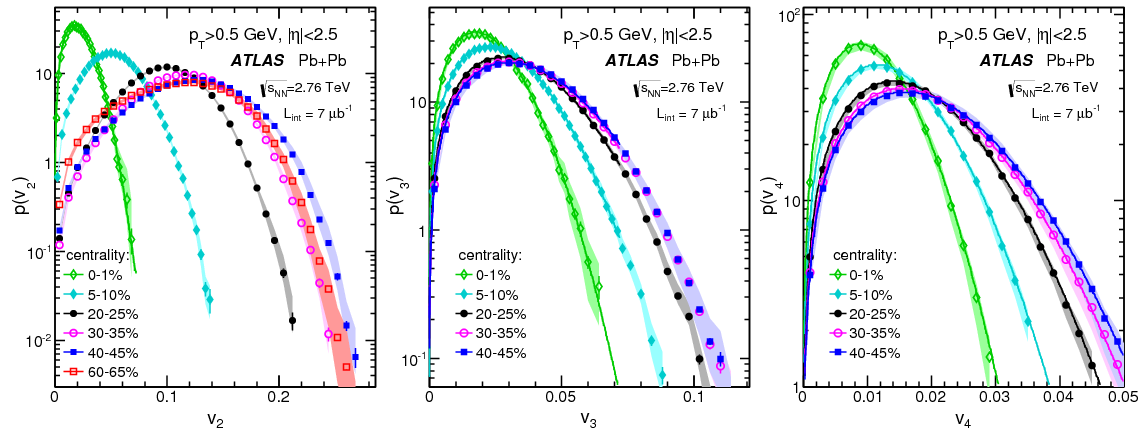
\includegraphics[width=3cm]{atlas-flows}};
      %\tikz\node [anchor=south west] {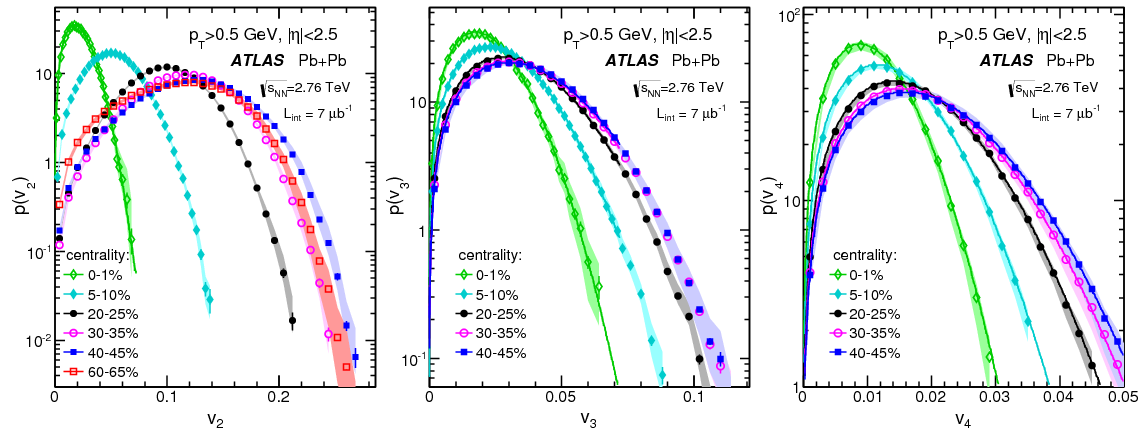
\includegraphics[width=3cm]{atlas-flows}};
      %\tikz\node at (0,0) {\includegraphics[width=3cm]{atlas-0}};
      %\vspace{2cm}\hspace{-.5cm}
      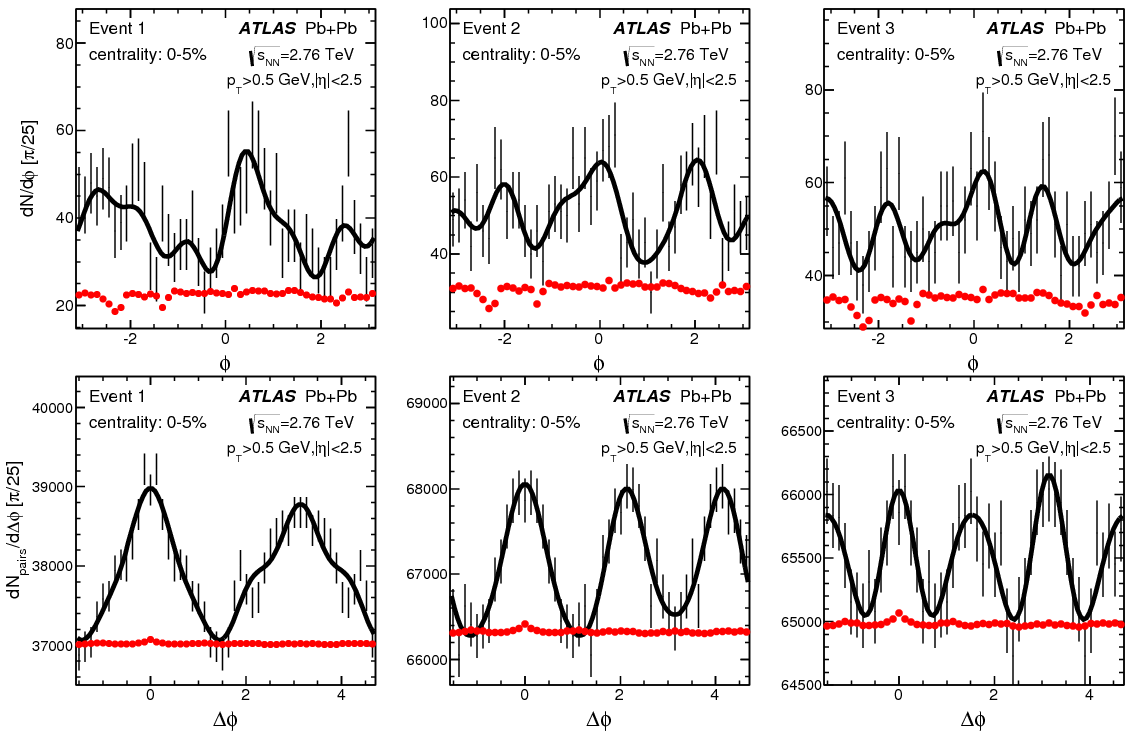
\includegraphics[width=3cm]{atlas-phi}
      \hspace{-.5cm}\vspace{-1cm}
      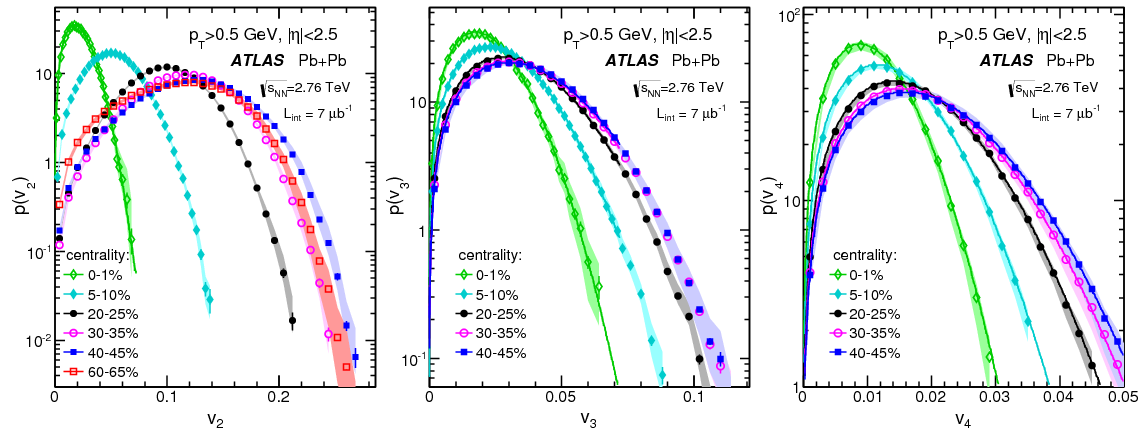
\includegraphics[width=3cm]{atlas-flows} \\[1cm]
      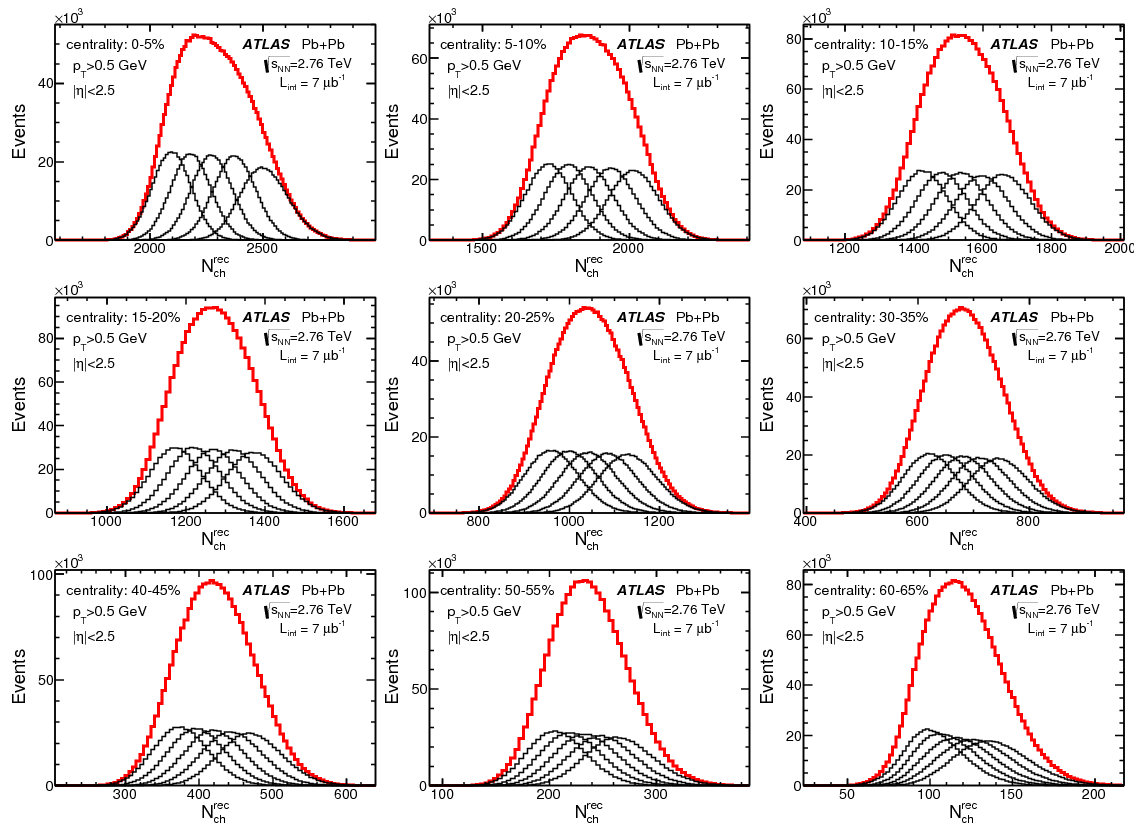
\includegraphics[width=3cm]{atlas-mult}
    };

    \draw[very thick,dashed,<->] (output) -- node[above] {\bf ?} (data); 
  \end{tikzpicture}
\end{frame}




\begin{frame}{The data}
  \begin{itemize}
    \item ATLAS event-by-event flow distributions for $v_2,v_3,v_4$.
    \item Shapes of distributions could provide a more sensitive probe of QGP properties than average flows.
    \item Reduce to three parameters by fitting to generalized gamma distribution
      \small
      \begin{equation*}
        f(x;s,a,c) = \frac{c}{s\,\Gamma(a)} \biggl( \frac{x}{s} \biggr)^{ac-1} \exp \biggl[ -\biggl( \frac{x}{s} \biggr)^c \biggr]
      \end{equation*}
  \end{itemize}

  \centering
  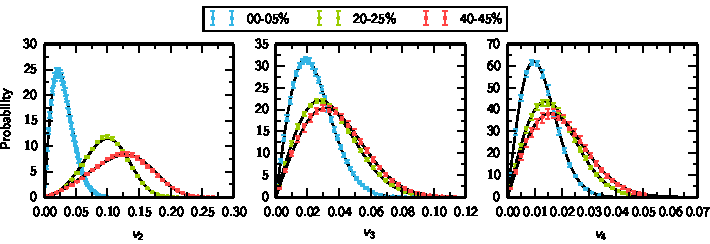
\includegraphics{atlasgengamma} %\\
  \flushright
  \tiny ATLAS collaboration, hep-ex/1305.2942
\end{frame}



\begin{frame}{The model}
  Modern version of the OSU+Duke hybrid model VISHNU (Viscous Hydro and UrQMD):
  \begin{itemize}
    \item MC-Glauber initial conditions {\tiny [H.-J.\ Drescher and Y.\ Nara, nucl-th/060512]}
    \item 2+1 viscous hydro {\tiny [H.\ Song and U.\ Heinz, nucl-th/0712.3715]}
    \item Cooper-Frye hypersurface sampler {\tiny [Z.\ Qiu and C.\ Shen]}
    \item UrQMD {\tiny [S.\ Bass \emph{et.\ al.}, nucl-th/9803035; M.\ Bleicher \emph{et.\ al.}, hep-ph/9909407]}
  \end{itemize}
  
  \vspace{.07\textheight}

  \centering
  \begin{tabular}{ll}
    \toprule
    Input parameters & Observables \\
    \midrule
    Normalization                           & \\
    WN/BC $\alpha$                          & $v_n$ distributions \\
    Thermalization time $\tau_0$            & Multiplicities \\
    Viscosity $\eta/s$                      & \ldots \\
    Shear stress relaxation time $\tau_\Pi$ & \\
    \bottomrule
  \end{tabular}

\end{frame}




\begin{frame}{Computer experiments with slow models}
  \begin{columns}
    \column{.6\textwidth}
    \begin{itemize}
      \item Run model at predetermined set of input-parameter points.
        \begin{itemize}
          \item Each parameter influences multiple observables.
          \item Must vary all parameters simultaneously.
        \end{itemize}
      \item Interpolate between points to complete parameter space.
      \item Calibrate the model:  determine parameters that optimally describe reality.
    \end{itemize}

    \column{.37\textwidth}
    \centering
    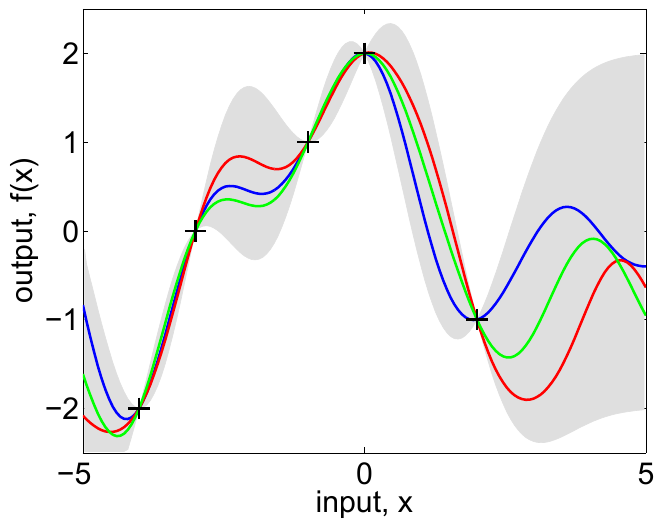
\includegraphics[width=\textwidth]{gpr2} \\
    \flushright\tiny \emph{Gaussian Processes for Machine Learning}, Rasmussen and Williams, 2006.
  \end{columns}
\end{frame}




\begin{frame}{Computer experiment design}
  \begin{itemize}
    \item Five centrality bins from 0--5\% to 40--45\%.
    \item 256 Latin-hypercube points across five input parameters.
    \item Running on Open Science Grid.
    \item Completed 1000-2000 events per centrality bin and input-parameter point.
      \begin{itemize}
        \item $\sim$1.9 million total
        \item $\sim$0.25 $\mu\text{b}^{-1}$  (ATLAS results based on 7 $\mu\text{b}^{-1}$)
      \end{itemize}
  \end{itemize}

  \bgs
  \begin{itemize}
    \item (5 centrality bins) $\times$ (3 flow coefficients) = 15 flow ``categories''
    \item $v_2$ 0--5\% and $v_2$ 40--45\% are representative.
  \end{itemize}
\end{frame}



\begin{frame}{Model flow distributions}
  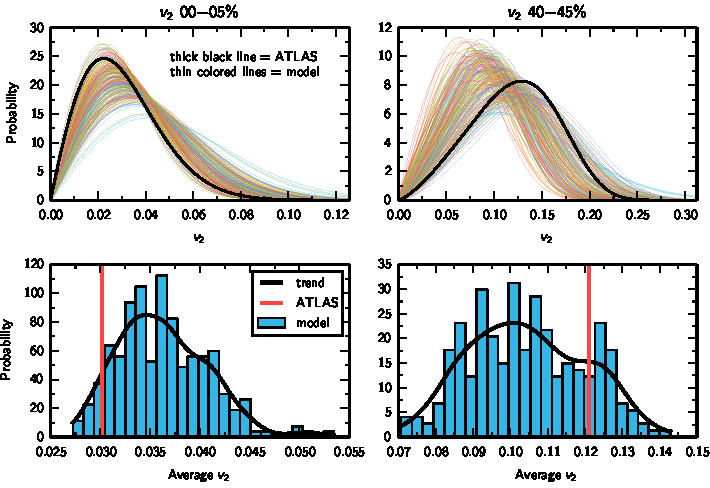
\includegraphics{allcurvesavgs}
\end{frame}


\begin{frame}{Comparing model and experimental distributions}
  \begin{columns}
    \column{.35\textwidth}
    \centering
    Kolmogorov-Smirnov test \\
    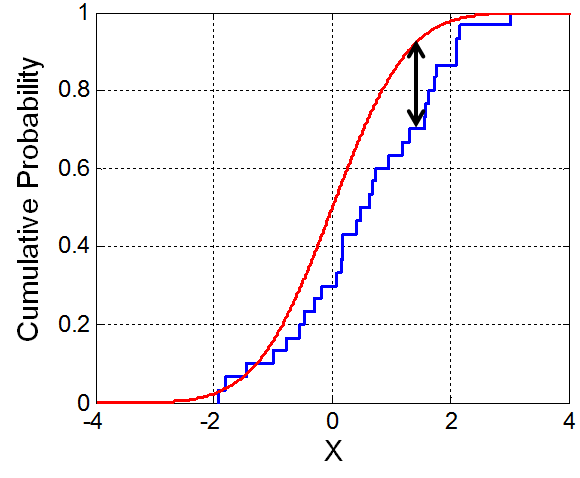
\includegraphics[width=\textwidth]{ks}
    \flushright
    \vspace{-1.5em}{\tiny Wikimedia commons} \\
    \centering
    \bgs
    \framebox{smaller KS $\implies$ better fit}

    \column{.6\textwidth}
    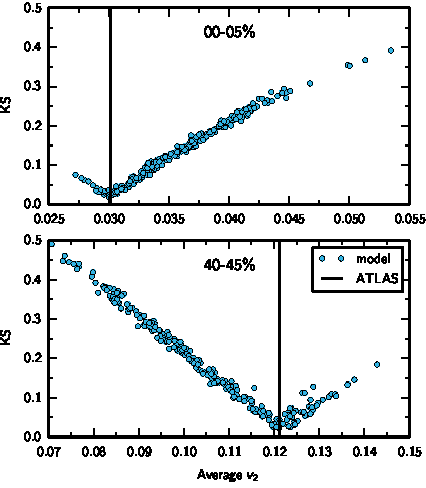
\includegraphics{ksvsavg}
  \end{columns}
\end{frame}



\begin{frame}{Input-output summary}
  \includegraphics<1>{scatters_v2_00-05}
  \includegraphics<2,3>{scatters_v2_40-45}
  \only<3>{
    \tikz[remember picture,overlay] \fill[draw=none,fill=black,opacity=.4] (current page.south west) ++(0,0) -- ++(7.79,0) --
    ++(0,3.70) -- ++(2.29,0) -- ++(0,-3.70) -- (current page.south east) -- ++(0,8.04) -- ++(-12.80,0) -- ++(0,-4.33) -- ++(.90,0) --
    ++(0,-2.85) -- ++(-.90,0) -- cycle;
  }
\end{frame}


\begin{frame}{Focusing on viscosity}
  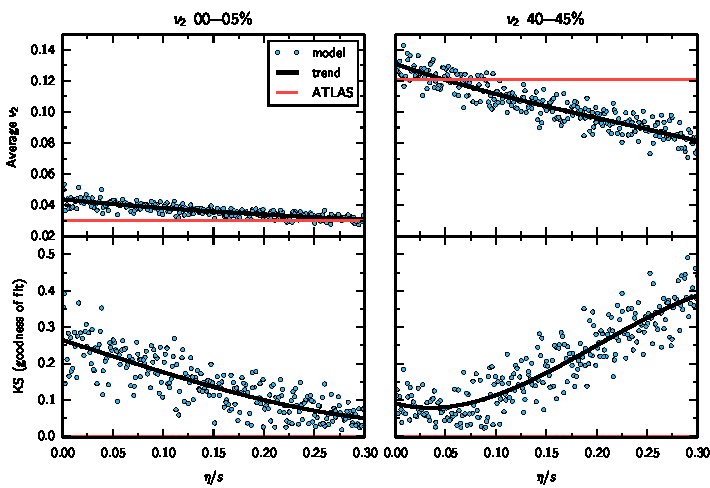
\includegraphics{avgksvsetas}
\end{frame}



\begin{frame}{Best fits}
  \begin{itemize}
    \item Split $\eta/s$ range into sub-ranges.
    \item Pick parameter point with best overall fit in each $\eta/s$ sub-range.
  \end{itemize}
  \centering
  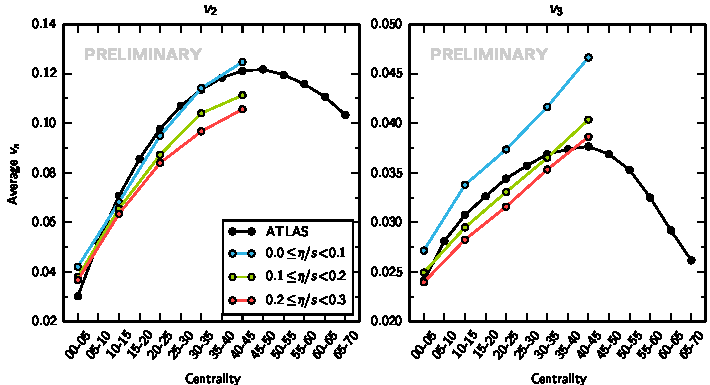
\includegraphics{bestavgvn}
\end{frame}





\begin{frame}{Summary \& outlook}
  \begin{columns}
    \column{.5\textwidth}

  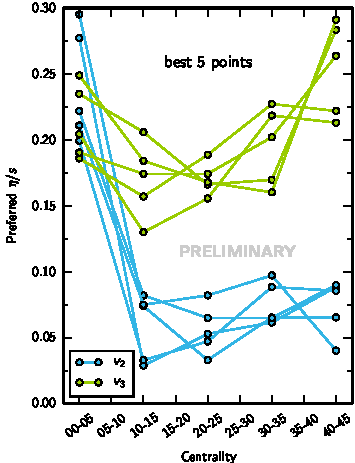
\includegraphics{bestetas}
    \column{.5\textwidth}
    
  \begin{itemize}
    \item $\eta/s$ compromise
      \begin{itemize}
        \item $\eta/s$ temperature dependence?
        \item Expand parameter space?
      \end{itemize}
    \item Quantitative statistical metrics
    \item Calibrate simultaneously on multiplicity
    \item Improved initial conditions (KLN, IP-Glasma)
  \end{itemize}
  \end{columns}
\end{frame}



\appendix


\begin{frame}[plain,noframenumbering]{}
  \centering
  \Large
  backup slides
\end{frame}

\begin{frame}{Latin-hypercube sampling}
  \begin{itemize}
    \item Optimally fills parameter space.
    \item Avoids clusters.
  \end{itemize}

  \centering
  \includegraphics<1>{lhs1}
  \includegraphics<2>{lhs2}
\end{frame}


\begin{frame}{Gaussian process emulators}
  \begin{itemize}
    \item Prior:  the model is a Gaussian process.
    \item Posterior:  Gaussian process conditioned on model outputs.
  \end{itemize}

  %\sms

  \begin{tikzpicture}
    \draw[very thick,->] (0,0) node[left,align=center] {\ \ prior \\ \includegraphics[width=.38\textwidth]{gpr1}} -- 
    node[above] {training} (2.0,0) node[right,align=center] {\ \ \ \ posterior \\ 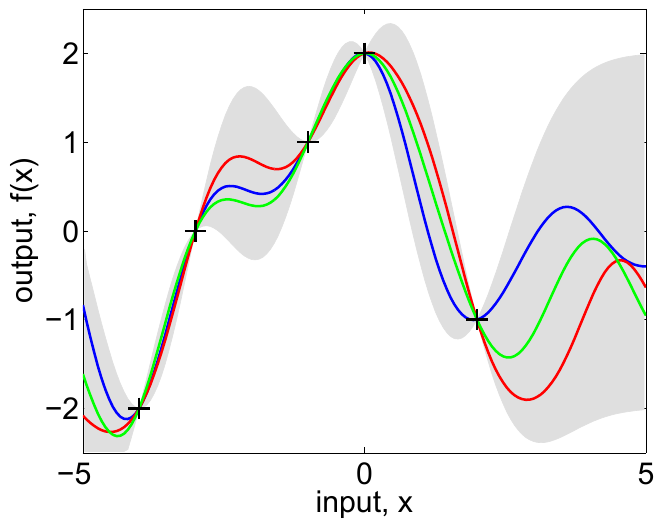
\includegraphics[width=.41\textwidth]{gpr2}};
  \end{tikzpicture}
  
  %\sms

  \begin{itemize}
    \item Emulator is a fast surrogate to the actual model.
      \begin{itemize}
        \item More certain near calculated points.
        \item Less certain in gaps.
      \end{itemize}
  \end{itemize}
\end{frame}


\begin{frame}{Testing $v_4$}
  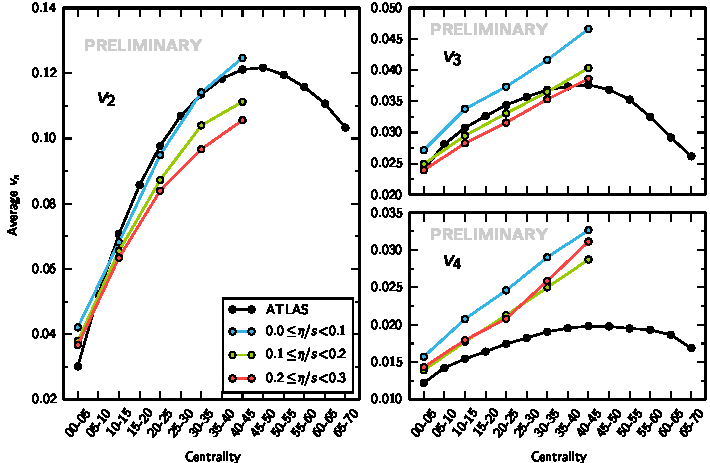
\includegraphics{bestavgvnwithv4}
\end{frame}


\begin{frame}{Multiplicity}
  \includegraphics<1>{scatters_mult_00-05}
  \includegraphics<2>{scatters_mult_40-45}
\end{frame}






\end{document}
